\section{Continuous Queries}
\label{sec:continuous}

MapReduce is often used to analyze streams of constantly-arriving
data, such as URL access logs~\cite{mapreduce-osdi} and system console
logs~\cite{sosp-mining}. Because of traditional constraints on MapReduce, this 
is done in large batches that can only provide periodic views of activity.
This introduces
significant latency into a data analysis process that ideally should run in 
near-real time. It is also
potentially inefficient: each new MapReduce job does not have access
to the computational state of the last analysis run, so this state
must be recomputed from scratch. The programmer can manually save the
state of each job and then reload it for the next analysis operation,
but this is labor-intensive.

Our pipelined version of Hadoop allows an alternative architecture:
MapReduce jobs that run \emph{continuously}, accepting new data as it
becomes available and analyzing it immediately. This allows for near-real-time
analysis of data streams, and thus
allows the MapReduce programming model to be applied to domains such
as environment monitoring and real-time fraud detection.

In this section, we describe how HOP supports continuous MapReduce
jobs, and how we used this feature to implement a rudimentary
cluster monitoring tool.

\subsection{Continuous MapReduce Jobs}
A bare-bones implementation of continuous MapReduce jobs is easy to
implement using pipelining. No changes are needed to implement
continuous map tasks: map output is already delivered to the
appropriate reduce task shortly after it is generated. We added an
optional ``flush'' API that allows map functions to force their current
output to reduce tasks. When a reduce task is unable to accept such data, the mapper framework
stores it locally and sends it at a later time. 
With proper scheduling of reducers, this API allows a map task to ensure that an output record is promptly sent to the appropriate
reducer.

To support continuous reduce tasks, the user-defined reduce function
must be periodically invoked on the map output available at that
reducer. Applications will have different requirements for how
frequently the reduce function should be invoked; possible choices
include periods based on wall-clock time, logical time (e.g., the
value of a field in the map task output), and the number of input rows
delivered to the reducer. The output of the reduce function can be
written to HDFS, as in our implementation of online
aggregation. However, other choices are possible; our prototype system
monitoring application (described below) sends an alert via email if
an anomalous situation is detected.

In our current implementation, the number of map and reduce tasks is
fixed, and must be configured by the user. This is clearly
problematic: manual configuration is error-prone, and many stream
processing applications exhibit ``bursty'' traffic patterns, in which
peak load far exceeds average load. In the future, we plan to add
support for elastic scaleup/scaledown of map and reduce tasks in
response to variations in load.

\subsubsection{Fault Tolerance}
In the checkpoint/restart fault-tolerance model used by Hadoop, mappers retain
their output until the end of the job to facilitate fast recovery from reducer
failures. In a continuous query context, this is infeasible, since mapper
history is in principle unbounded.  However, many continuous reduce functions
(e.g., 30-second moving average) only require a suffix of the map output stream.
This common case can be supported easily, by extending the \JT\ interface to
capture a rolling notion of reducer consumption.  Map-side spill files are
maintained in a ring buffer with unique IDs for spill files over time. When a
reducer commits an output to HDFS, it informs the \JT\ about the \emph{run} of
map output records it no longer needs, identifying the run by spill file IDs and
offsets within those files.  The \JT\ can then tell mappers to garbage collect
the appropriate data.

In principle, complex reducers may depend on very long (or infinite) histories of map records to accurately reconstruct their internal state.  In that case, deleting spill files
from the map-side ring buffer will result in potentially inaccurate recovery after faults.  Such scenarios can be handled by having reducers checkpoint internal state to HDFS, along with markers for the mapper offsets at which the internal state was checkpointed.  The MapReduce framework can be extended with APIs to help with state serialization and offset management, but it still presents a programming burden on the user to correctly identify the sensitive internal state.  That burden can be avoided by more heavyweight process-pair 
techniques for fault tolerance, but those are quite complex and use significant resources~\cite{flux-ft}.  In our work to date we have focused on cases where reducers can be recovered from a reasonable-sized history at the mappers, favoring minor extensions to the simple fault-tolerance approach used in Hadoop.

\subsection{Prototype Monitoring System}
Our monitoring system is composed of \emph{agents} that run on each monitored
machine and record statistics of interest (e.g., load average, I/O operations
per second, etc.). Each agent is implemented as a continuous map task: rather
than reading from HDFS, the map task instead reads from various system-local
data streams (e.g., \texttt{/proc}).

Each agent forwards statistics to an \emph{aggregator} that is implemented as a
continuous reduce task. The aggregator records how agent-local statistics evolve
over time (e.g., by computing windowed-averages), and compares statistics
between agents to detect anomalous behavior. Each aggregator monitors the agents
that report to it, but might also report statistical summaries to another
``upstream'' aggregator. For example, the system might be configured to have an
aggregator for each rack and then a second level of aggregators that compare
statistics between racks to analyze datacenter-wide behavior.

\subsection{Evaluation}
\begin{figure}[t]
%%\begin{minipage}{0.5\linewidth}
  \centering
  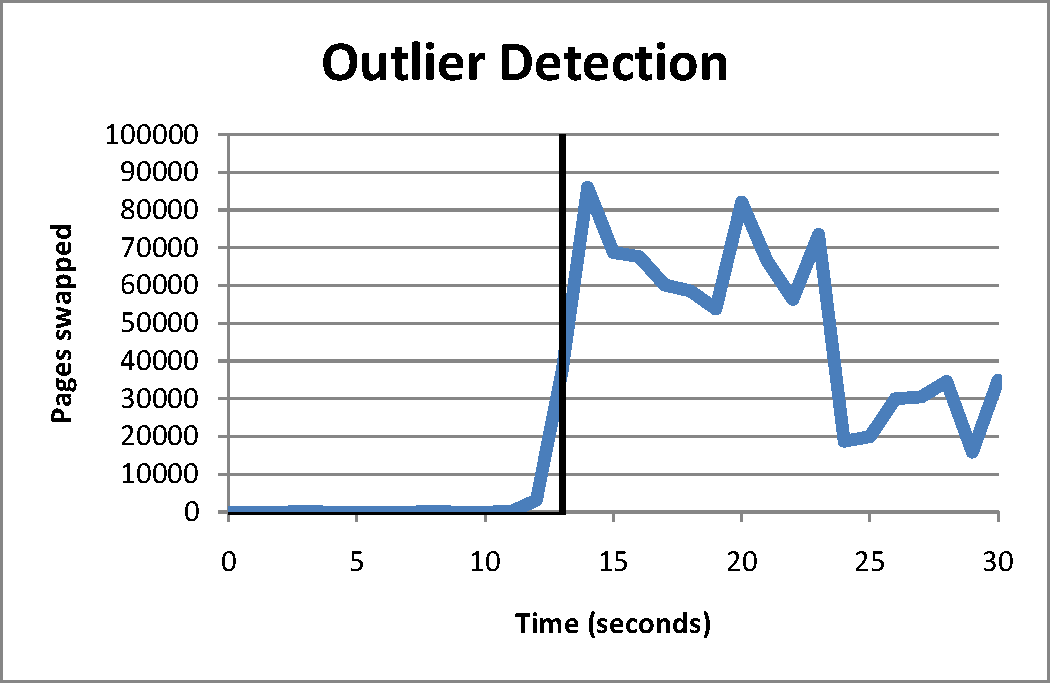
\includegraphics[width=0.95\linewidth]{eval/continue.pdf}
%%\end{minipage}
  \caption{Number of pages swapped over time on the thrashing host, as reported
    by \texttt{vmstat}.  The vertical line indicates the time at which the alert
    was sent by the monitoring system.}
\label{fig:outlier}
\end{figure}

To validate our prototype system monitoring tool, we constructed a
scenario in which one member of a MapReduce cluster begins thrashing
during the execution of a job. Our goal was to test how quickly our
monitoring system would detect this behavior. The basic mechanism is
similar to an alert system one of the authors implemented at an
Internet search company.

We used a simple load metric (a linear combination of CPU utilization,
paging, and swap activity). The continuous reduce function maintains
windows over samples of this metric: at regular intervals, it
compares the 20 second moving average of the load metric for each host
to the 120 second moving average of all the hosts in the cluster
\emph{except} that host.  If the given host's load metric is more
than two standard deviations above the global average, it is
considered an outlier and a tentative alert is issued.  To dampen
false positives in ``bursty'' load scenarios, we do not issue an alert
until we have received 10 tentative alerts within a time window.

We deployed this system on an EC2 cluster consisting of 7 ``large''
nodes (large nodes were chosen because EC2 allocates an entire
physical host machine to them). We ran a wordcount job on the 5.5GB Wikipedia
data set, using 5 map tasks and 2 reduce tasks (1 task per host). After
the job had been running for about 10 seconds, we selected a node
running a task and launched a program that induced thrashing.

We report detection latency in Figure~\ref{fig:outlier}. The vertical bar
indicates the time at which the monitoring tool fired a (non-tentative)
alert. The thrashing host was detected very rapidly---notably faster than the
5-second {\TT}-{\JT} heartbeat cycle that is used to detect straggler tasks in
stock Hadoop. We envision using these alerts to do early detection of stragglers
within a MapReduce job: HOP could make scheduling decisions for a job by running
a secondary continuous monitoring query. Compared to out-of-band monitoring
tools, this economy of mechanism---reusing the MapReduce infrastructure for
reflective monitoring---has benefits in software maintenance and system
management.
